
\chapter{Empirical Analysis in Native Containers}

  The list of questions mentioned in section:\ref{section_questions} are questions of interest that would help us understand the existing 
memory management techniques better. We have tried answer the listed questions by mapping them into appropriate experiments. Inferences 
were drawn based on the observations in the experiments. There were 3 different categories of questions we have tried to answer using 
empirical analysis in a native container environment as listed below,
  
  \begin{enumerate}
    \item Verify the correctness of our hypotheses
    \item Understand parts of memory management for which hypothesis couldn't be drawn
    %\item Understand the implications of existing memory management on application performance
  \end{enumerate}
  
  The configuration in Table:\ref{table_native_base} is the base configuration for all experiments in this section. Any changes the base 
configuration has been mentioned in the procedure of each of the experiment.

    \begin{table}	 
      \begin{center}
	\begin{tabular}{ l | c | c }
	  & Container-1 (M1) & Container-2 (M2) \\ 
	  \hline
	  \hline
	  Size of VM & \multicolumn{2}{c}{2 GB} \\	      
	  \hline
	  Workload & Memory Hogger & Memory Hogger \\
	  \hline
	  Hard Limit & 1000 MB & 1000 MB \\  
	  \hline
	  Soft Limit & 150 MB & 150 MB \\  
	  \hline
	  Memory Usage & 500 MB & 500 MB \\
	  \hline
	  Exceed & 350 MB & 350 MB \\
	  \hline 
	  External Pressure & \multicolumn{2}{l}{ 200 - 400 - 600 - 800 - 1000 MB} \\
	\end{tabular}	    
	\caption{Base Configuration}
	\label{table_native_base}
      \end{center}
    \end{table}
    
    Most experiments involved setting up of 2 containers. Workloads were used to introduce system memory pressure from containers. At 
this point there was no memory pressure in the system (free memory was still available). Now the external pressure using Stress was 
introduced after about 20s which created memory pressure in the system that triggered reclamation. The external pressure kept on increasing 
by 200 MB in intervals of 40s. Each interval had a gap of 10s for memory to be reassigned to containers.
  
  %For the sake of simplicity, questions of category 1 and 2 were answered using the native testbed using synthetic workloads as described 
%in section:\ref{section_testbed_native}. Questions of category 3 were answered using the derivative testbed using real workloads as 
%described in section:\ref{section_testbed_derivative}

  \section{Verification of hypotheses}
    
    The following set of experiments were done to establish the hypotheses we purposed actually hold good 
    
    \subsection{Exp-1: All containers exceed}
	
	\subsubsection{Hypothesis:} 
	  \begin{enumerate}
	    \item SMR (Soft Memory Reclamation) purely based on exceed value of the container
	    \item Majority of reclamation when containers exceed occurs using SMR
	    \item Containers that exceed equally are iteratively targeted
	  \end{enumerate} 
	
	\subsubsection{Procedure:}
	  To demonstrate the correctness of our hypothesis we the base configuration described in Table:\ref{table_native_base} and change 
the usage to 700 MB and soft limit to 350 MB there by simulating an scenario where \textbf{Both containers exceeded by the same values}.
	
      	\begin{figure}
	  \centering
	  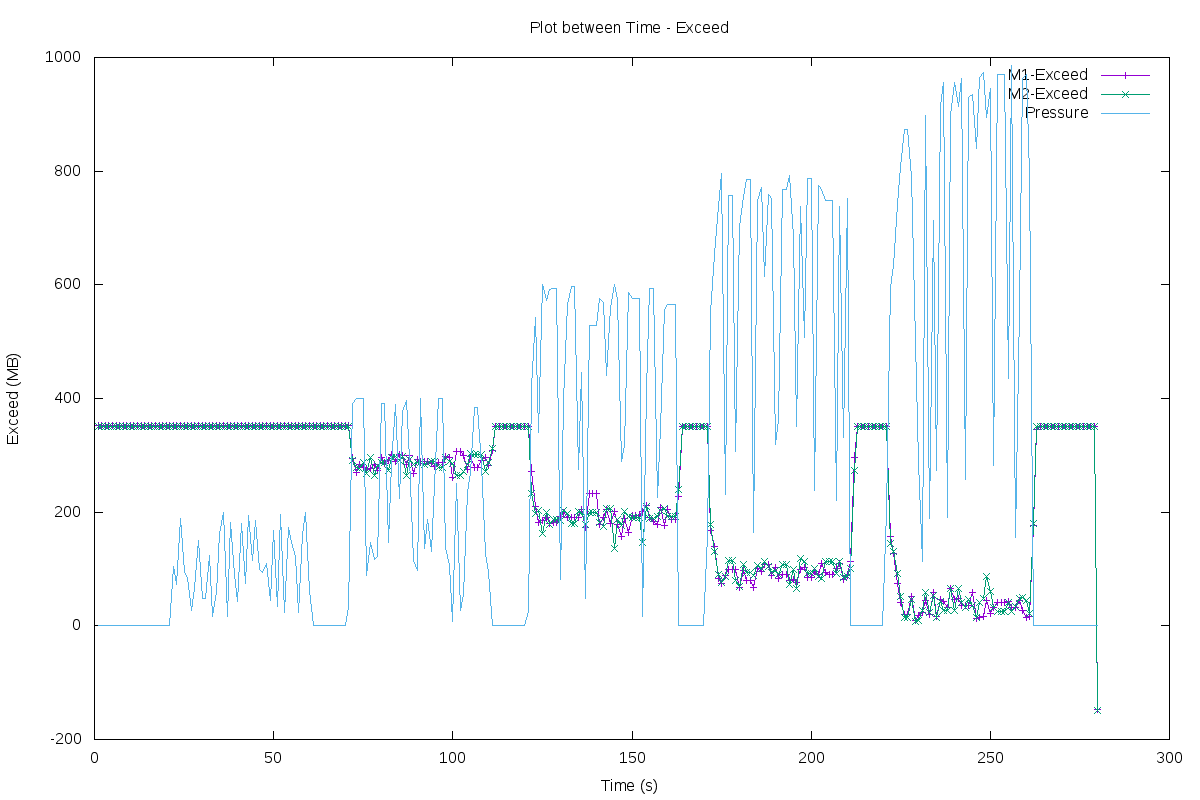
\includegraphics[width=0.8\textwidth]{images/experimentation/exceed_only/1/Exceed.png}
	  \caption{Memory Exceed Plot for Exp-1}
	  \label{img_exceed_only_1_exceed}
	\end{figure}
	
	\begin{figure}
	  \centering
	  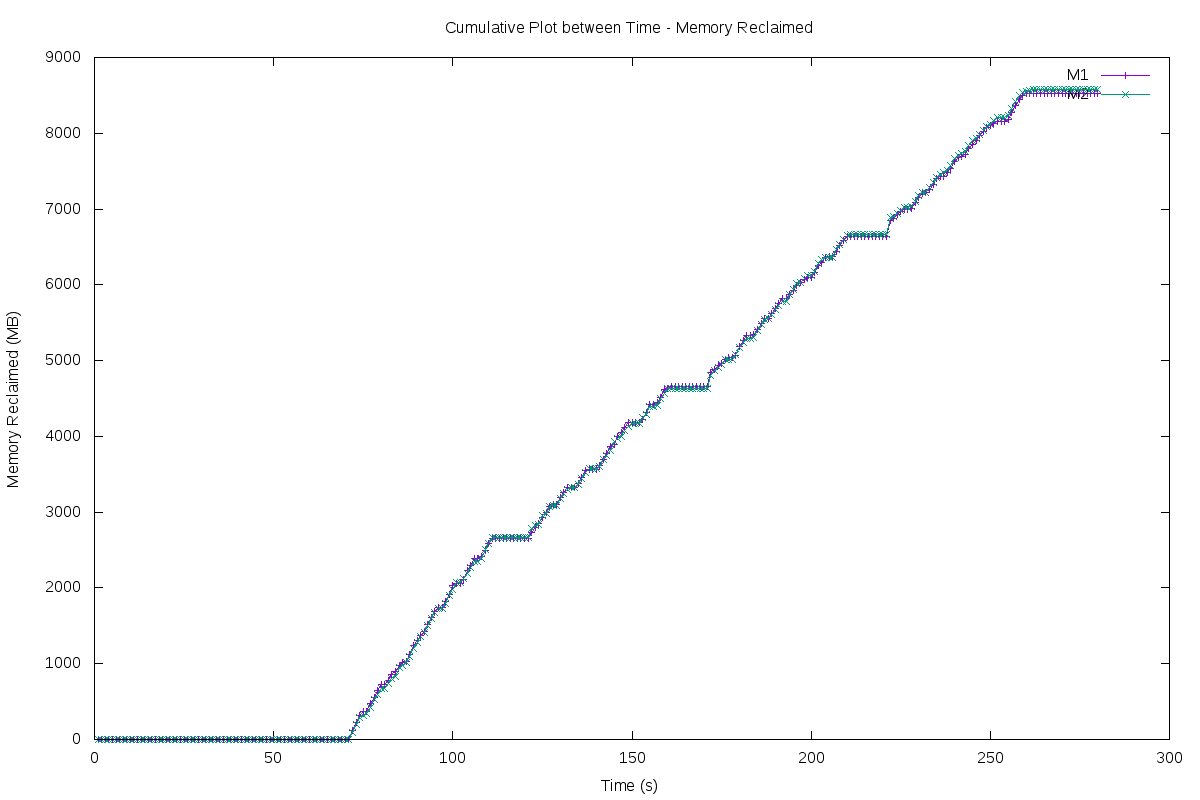
\includegraphics[width=0.8\textwidth]{images/experimentation/exceed_only/1/Memory_Reclaimed.png}
	  \caption{Soft Memory Reclaimed Plot for Exp-1}
	  \label{img_exceed_only_1_smr}
	\end{figure}
	
	\begin{figure}
	  \centering
	  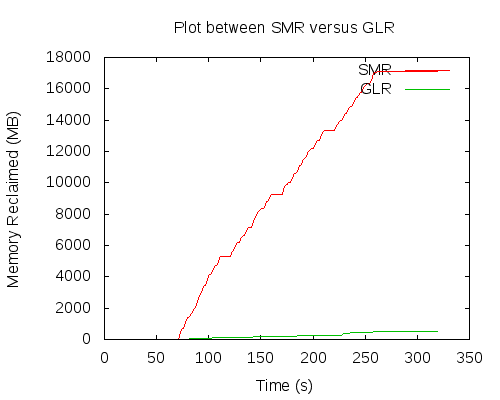
\includegraphics[width=0.8\textwidth]{images/experimentation/smr_glr/1/compare.png}
	  \caption{SMR versus GLR for Exp-1}
	  \label{img_exceed_only_1_compare}
	\end{figure}
	
	\subsubsection{Observations:}
	
	  \begin{itemize}
	    \item As seen from Fig:\ref{img_exceed_only_1_exceed}, Fig:\ref{img_exceed_only_1_smr} - memory reclaimed from containers 
iteratively from one after the other as their exceeds are same.
	    \item Fig:\ref{img_exceed_only_1_compare} shows how most reclamation when containers exceed occurs using SMR however it is seen 
that there is minimum reclamation occurring using GLR as well.
	  \end{itemize}

	\subsubsection{Inference:}	
	  \begin{itemize}
	    \item SMR is purely based on exceed value.
	    \item Most reclamation when containers exceed occurs using SMR, however the GLR kicks in every reclamation request to evict any 
inactive page cache pages in the system (may/may not belong to container).
	    \item Containers that exceed equally are iteratively target for reclamation one after the other.
	  \end{itemize}

    
    \subsection{Exp-2: None of the containers exceed}
   
    \subsubsection{Hypothesis:}
      Does our hypotheses of reclamation below soft limits falling back to native system reclamation hold good ?
      
    \subsubsection{Procedure:}  
      To test the reclamation patterns in containers below soft limits, we created containers as mentioned in Table:\ref{table_native_base} 
and changed soft limits of both containers to 1000 MB there by making the current \textbf{usage of both containers below soft limits}. We 
used hooks in the kernel code to track requests satisfied by soft memory reclamation (SMR) and global LRU based reclaimation (GLR).
     
      \begin{figure}
	\centering
	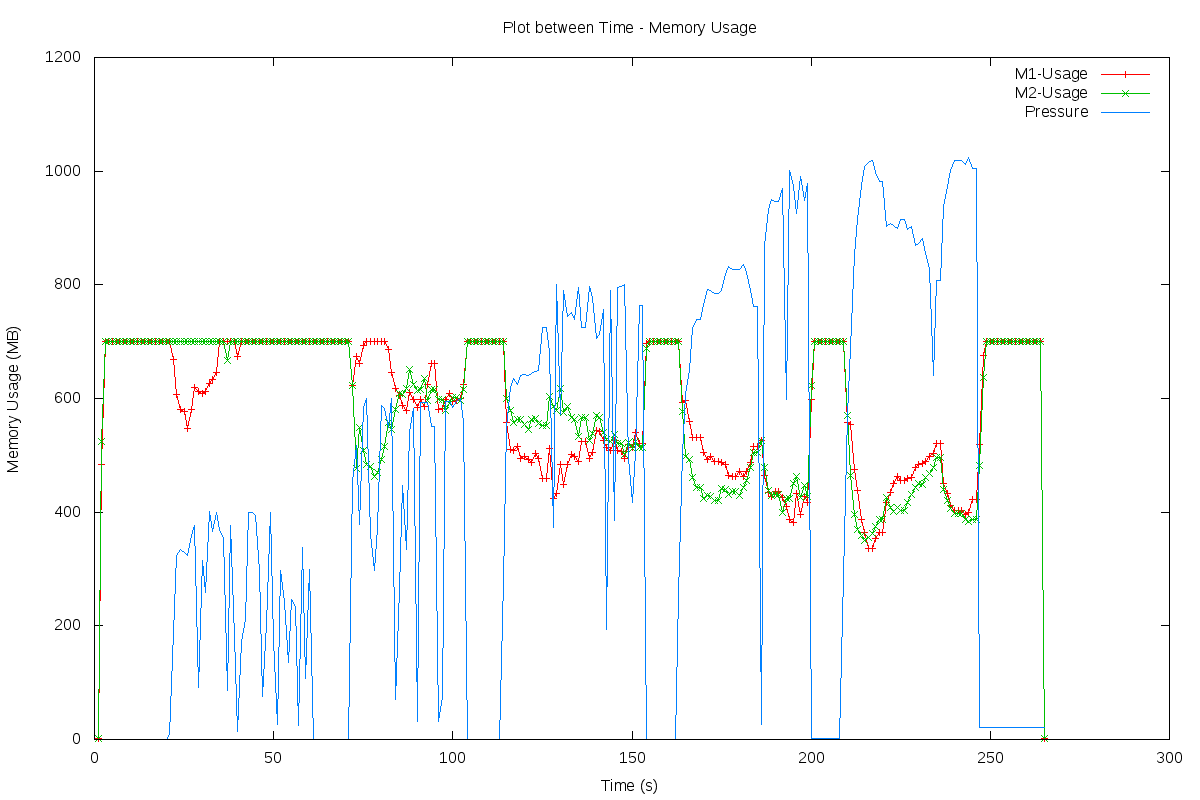
\includegraphics[width=0.8\textwidth]{images/experimentation/global_lru/no_sl_mu.png}
	\caption{Memory Usage Plot for Exp-2}
	\label{img_no_sl_mu}
      \end{figure}
      
      \begin{figure}
	\centering
	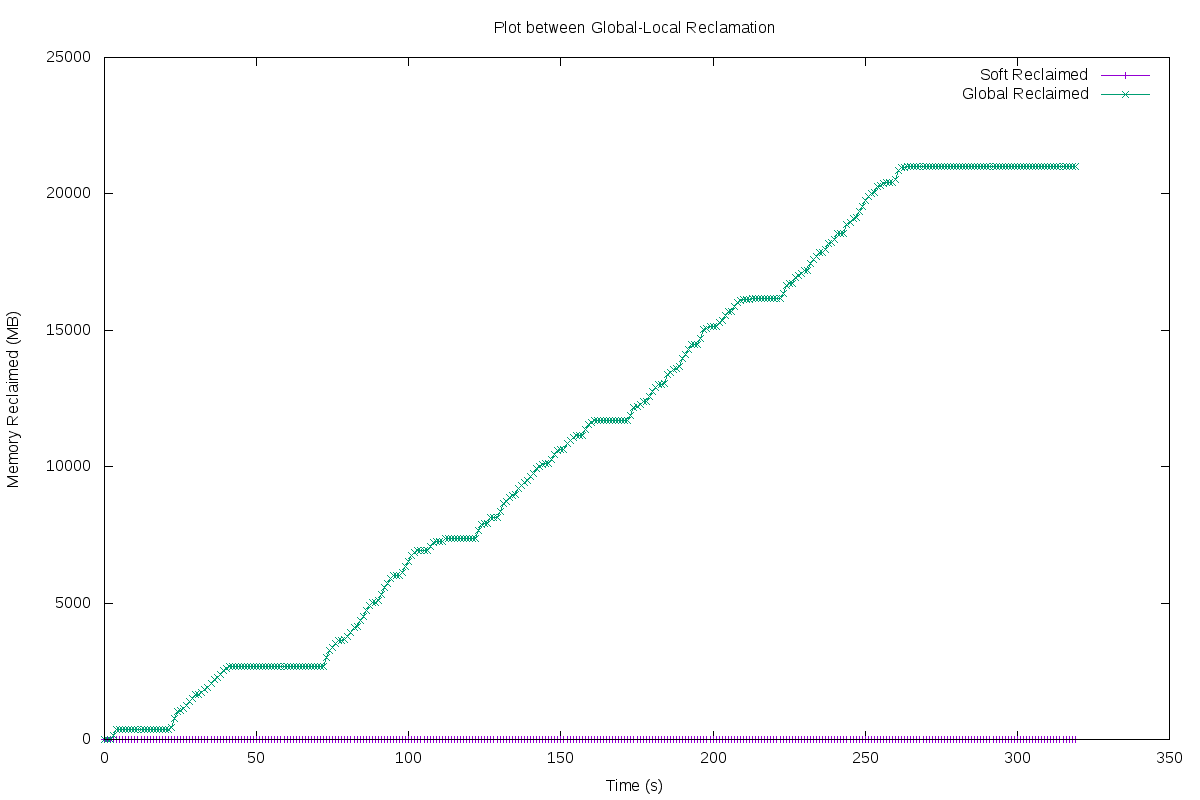
\includegraphics[width=0.8\textwidth]{images/experimentation/global_lru/no_sl_global_vs_local.png}
	\caption{SMR versus GLR Plot for Exp-2}
	\label{img_no_sl_global_vs_local}
      \end{figure}
      
      \subsubsection{Inference:}
	\begin{itemize}
	  \item As seen from Fig:\ref{img_no_sl_mu}, there is no hand-in-hand reclamation that occurs to containers below their soft 
limits although the containers are running the same workload, unlike hand in hand reclamation that occurs in memory usage above soft limits.
	  \item Since both containers are below SL, all reclamation is occurring using the GLR (Global LRU based reclamation) as seen by 
Fig:\ref{img_no_sl_global_vs_local}
	\end{itemize}

      \subsubsection{Conclusion:}
	\begin{itemize}
	  \item Containers with memory usage below soft limits reclamation falls back to native system GLR.
	  \item Reclamation using GLR is haphazard and there is no control over it. 
	\end{itemize}

%%%%%%%%%%%%%%%%%%%%%%%%%%%%%%%%%%%%%%%%%%%%%%%%%%%%%%%%%%%%%%%%%%%%%%%%%%%%%%%%%%%%%%%%%%%%%%%%%%%%%%%%%%%%%%%%%%%%%%%%%%%%%%%%%%%%%%
  
  \section{Understand Memory Reclamation}
  
    This section presents list of experiments to answer the list of questions for which hypotheses couldn't be drawn. 
  
    \subsection{Exp-3: Affect of system memory pressure on Reclamation}
	
	\subsubsection{Question:} 
	   In what ratio does SMR and GLR vary based on system memory pressure ? Does only SMR occur when container exceed is more than 
reclamation request ?
	
	\subsubsection{Procedure:}
	  To find out the amount of memory reclaimed using SMR and GLR we took our base configuration as in Table:\ref{table_native_base}. 
We run one experiment (Exp-3a) with base configuration and note its reclamation pattern. We run another experiment (Exp-3b) by increasing 
its external pressure from 1000-1400 MB in increments of 100MB over intervals of 50s.
	 
	
	\begin{figure}
	  \centering
	  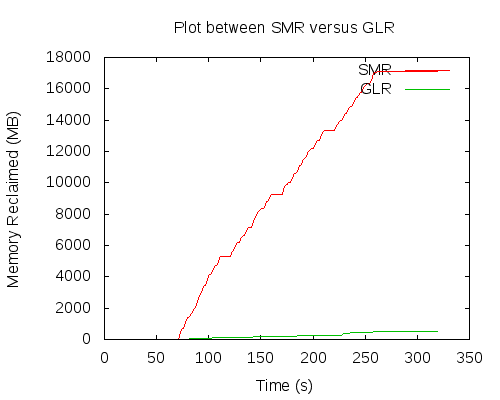
\includegraphics[width=0.8\textwidth]{images/experimentation/smr_glr/1/compare.png}
	  \caption{SMR versus GLR for Exp-3a}
	  \label{img_smr_glr_1_compare}
	\end{figure}
	
	\begin{figure}
	  \centering
	  \includegraphics[width=0.8\textwidth]{images/experimentation/smr_glr/2/compare.png}
	  \caption{SMR versus GLR for Exp-3b}
	  \label{img_smr_glr_2_compare}
	\end{figure}
	
	  
	\subsubsection{Observations:}
	
	  \begin{itemize}
	    \item With lesser external pressure most reclamation is satisfied by SMR as shown in Fig:\ref{img_smr_glr_1_compare} with 
98.1\% of requests satisfied by SMR.
	    \item As pressure increases, more and more reclamation is directed to GLR as shown in Fig:\ref{img_smr_glr_2_compare} now 
	    with 87.1\% (lesser) requests satisfied by SMR and the rest satified by GLR.
	    \item Notice how GLR increase as pressure increases from left to right of both plots.
	  \end{itemize}

	\subsubsection{Inference:}
	  \begin{itemize}
	    \item Both SMR and GLR occur simultaneously when containers exceed with even small reclamation requests. 
	    \item The global policy tries to satisfy most of the request through SMR, but as the reclamation demand increases it 
depends more on  the GLR.
	  \end{itemize}
  
    \subsection{Exp-4: Memory Reclaimed in a single SMR request}
	
	\subsubsection{Question:} 
 	  How much of memory is reclaimed from a container in a single reclamation SMR request ?
	
	\subsubsection{Procedure:}
	  We took our base configuration as described in Table:\ref{table_native_base}. However we ran two workloads in this case - Memory 
Hogger (Exp-4a) and File Hogger (Exp-4b) workloads on it as native theory suggests that containers with page cache pages might be 
victimized at larger the way it occurs with GLR.	
	
	\begin{figure}
	  \centering
	  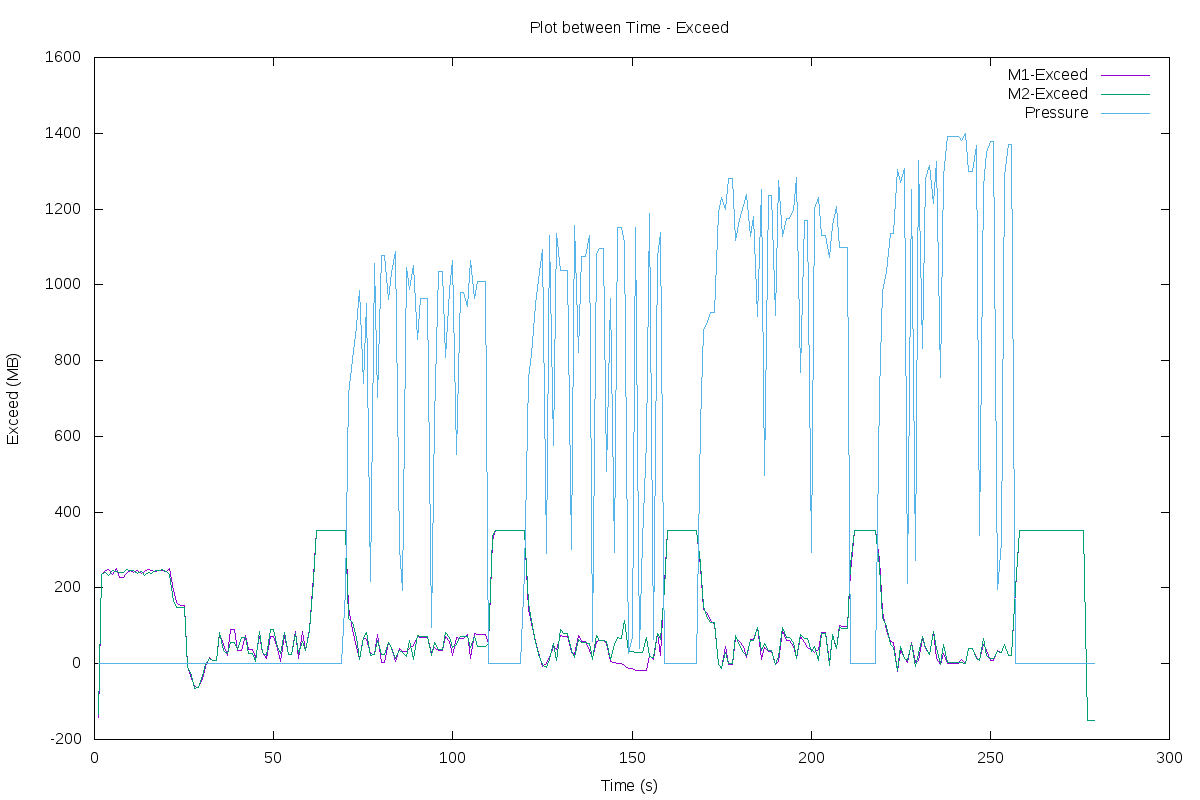
\includegraphics[width=0.8\textwidth]{images/experimentation/workload/1/Exceed.png}
	  \caption{Exceed plot for Experiment-4a}
	  \label{img_workload_1_exceed}
	\end{figure}
	
	\begin{figure}
	  \centering
	  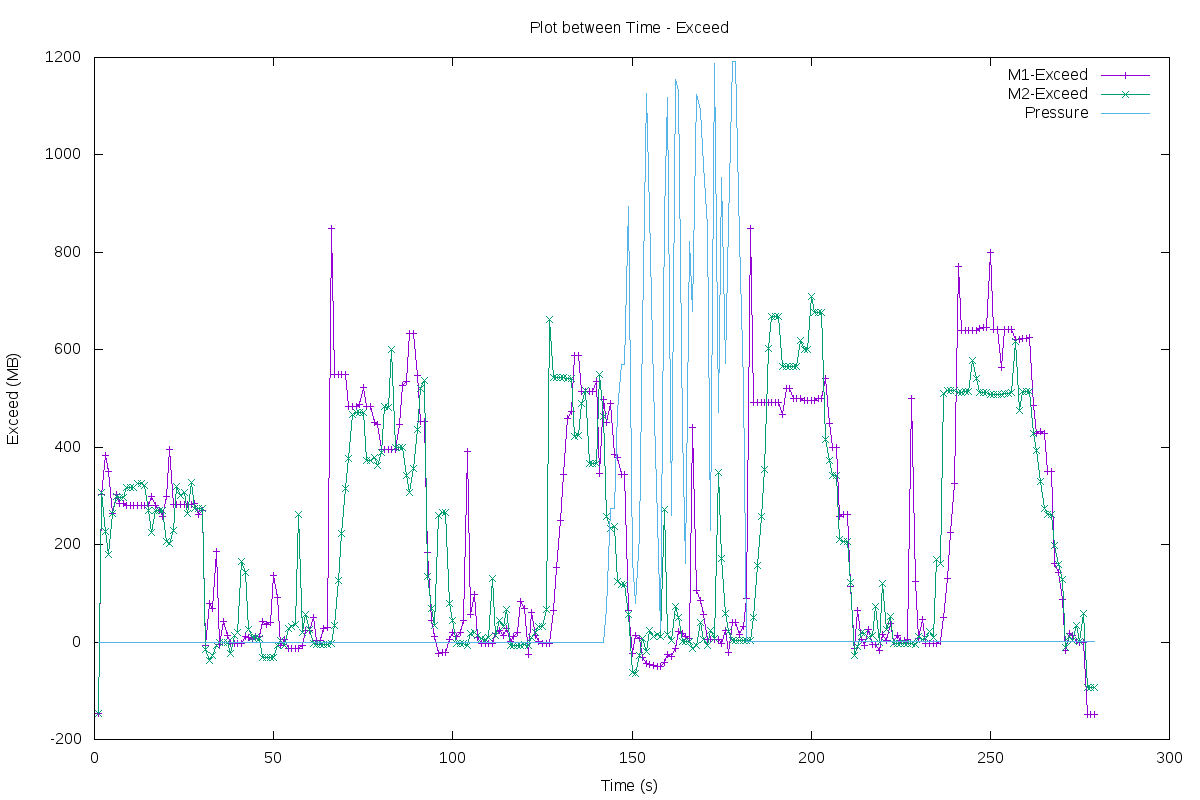
\includegraphics[width=0.8\textwidth]{images/experimentation/workload/2/Exceed.png}
	  \caption{Exceed plot for Experiment-4b}
	  \label{img_workload_2_exceed}
	\end{figure}	
	  
	\subsubsection{Observations:}
	
	\begin{itemize}
	  \item The exceed goes hand in hand as expected but with larger deviation in Fig:\ref{img_workload_1_exceed} and 
Fig:\ref{img_workload_2_exceed}
	  \item The larger deviation can be accounted to larger reclamation chunks in workloads that have page cache pages similar to how 
reclamation targets page cache pages in native system
	  \item Further empirical analysis of the reclamation chucks gave us the reclamation chucks to be 
	      \begin{center}
		  Reclamation chuck = Anonymous memory pages (\textless 25MB) + Page cache pages
	      \end{center}
	      In both cases pages from inactive zones were reclaimed before trying to reclaim from active lists.
	\end{itemize}

	\subsubsection{Inference:}
	
	\begin{itemize}
	  \item Workloads with page cache pages are reclaimed at larger chunks per SMR request
	\end{itemize}
      
      \subsection{Exp-5: Affect of Soft Limit on Reclamation}
	\label{soft_limit}
	
	\subsubsection{Question:} 
	  In what ratio does SMR and GLR vary based on container soft limits ?
	
	\subsubsection{Procedure:}
	  We took our base configuration as described in Table:\ref{table_native_base}. However we ran the experiments twice, 
once with the default soft limits that is 150 MB (Exp-5a), and then we doubled the soft limits to 300 MB (Exp-5b) and made our observations.
		
	\begin{figure}
	  \centering
	  \includegraphics[width=0.8\textwidth]{images/experimentation/sl_vary/1/compare.png}
	  \caption{SMR versus GLR for Exp-5a}
	  \label{img_sl_vary_1_compare}
	\end{figure}
	
	\begin{figure}
	  \centering
	  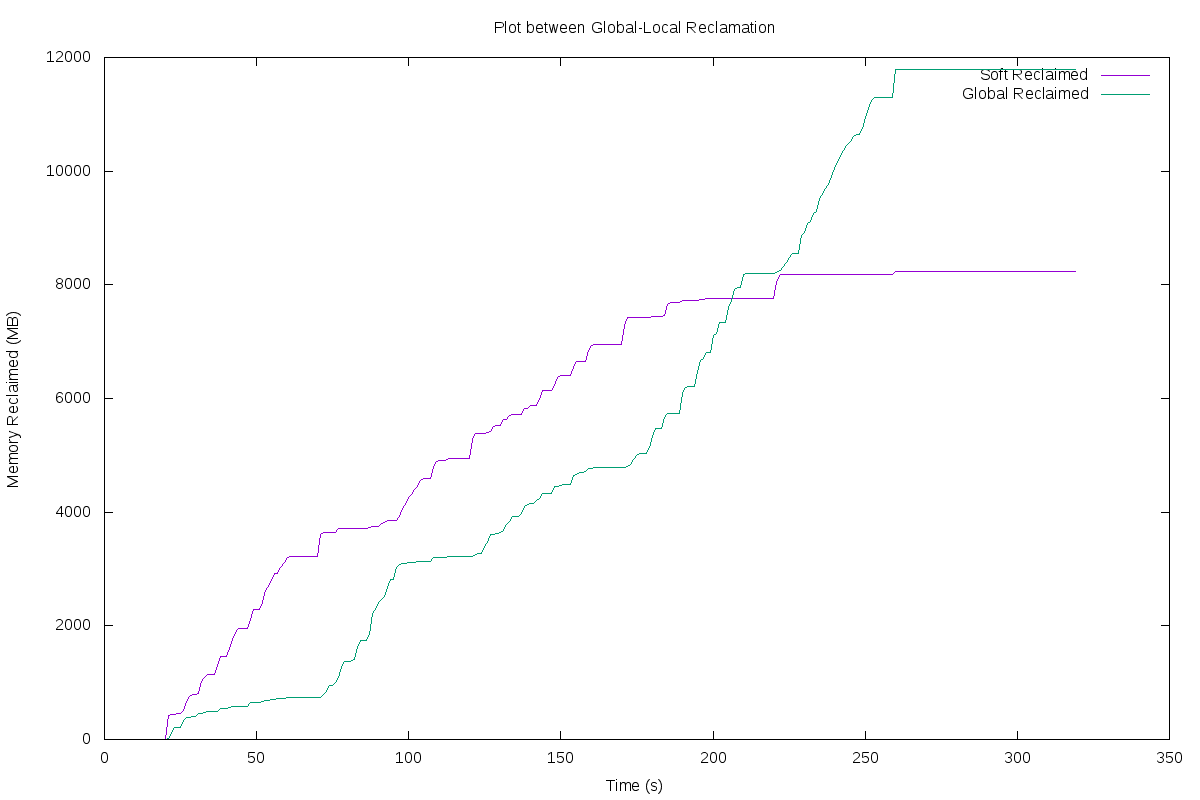
\includegraphics[width=0.8\textwidth]{images/experimentation/sl_vary/2/compare.png}
	  \caption{SMR versus GLR for Exp-5b}
	  \label{img_sl_vary_2_compare}
	\end{figure}	
	
	\begin{figure}
	  \centering
	  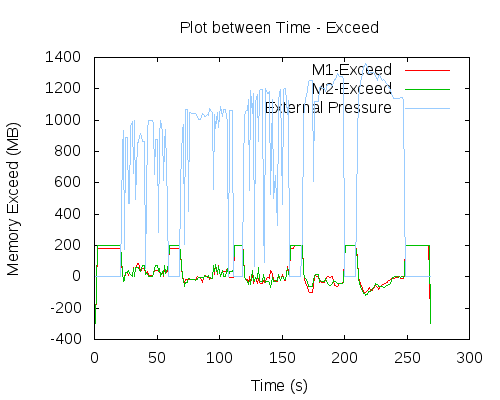
\includegraphics[width=0.8\textwidth]{images/experimentation/sl_vary/2/Exceed.png}
	  \caption{Exceed plot for Exp-4b}
	  \label{img_sl_vary_2_exceed}
	\end{figure}
	  
	\subsubsection{Observations:}
	
	  \begin{itemize}
	  \item Fig:\ref{img_sl_vary_1_compare} shows memory reclaimed using SMR (88.1\%) in with lower soft limits is higher than the 
memory that is reclaimed using SMR (41.1\%) with higher soft limits as shown in Fig:\ref{img_sl_vary_2_compare}. 
	  \item This occurs as the higher soft limits allows lesser opportunities for SMR and more for GLR.
	  \item Fif:\ref{img_sl_vary_2_exceed} shows how container exceeds can drop below 0 which indicates that the container usage is 
going below SL.
	\end{itemize}

	\subsubsection{Inference:}
	
	\begin{itemize}
	  \item Higher soft limits invokes GLR more frequently
	  \item Soft limit is not an absolute guarantee, it merely provides more stability to the minimum memory promised to a container 
	\end{itemize}
	
%%%%%%%%%%%%%%%%%%%%%%%%%%%%%%%%%%%%%%%%%%%%%%%%%%%%%%%%%%%%%%%%%%%%%%%%%%%%%%%%%%%%%%%%%%%%%%%%%%%%%%%%%%%%%%%%%%%%%%%%%%%%%%%%%%%%%%%%%%%
  
  \section{Key Insights}
    
    Here are the list of key implications that were derivative from running the above experiments in an synthetic environment. We have 
classified it based on the scenarios as discussed earlier.
    
    \subsection{All containers exceed}
    \begin{enumerate}
      \item When containers usage are above soft limits most reclamation occurs using SMR, however the GLR kicks in every reclamation 
request to evict any  inactive page cache pages in the system (may/may not belong to container).      
      \item SMR is purely based on exceed value of a container.
      \item Workloads with page cache pages are reclaimed at larger chunks per SMR request
      \item Containers that exceed equally are iteratively target for reclamation one after the other.
      \item Both SMR and GLR occur simultaneously when containers exceed with even small reclamation requests.      
    \end{enumerate}
    
    \subsection{None of the containers exceed}
    \begin{enumerate}
      \item Containers with memory usage below soft limits reclamation falls back to native system GLR.
      \item Reclamation using GLR is haphazard and there is no control over it. 
    \end{enumerate}
    
    \subsection{A few containers exceed, but the others don’t}
    \begin{enumerate}
      \item Soft limit is not an absolute guarantee, it merely provides more stability to the minimum memory promised to a container.
    \end{enumerate}

  
